%Copyright 2014 Jean-Philippe Eisenbarth
%This program is free software: you can 
%redistribute it and/or modify it under the terms of the GNU General Public 
%License as published by the Free Software Foundation, either version 3 of the 
%License, or (at your option) any later version.
%This program is distributed in the hope that it will be useful,but WITHOUT ANY 
%WARRANTY; without even the implied warranty of MERCHANTABILITY or FITNESS FOR A 
%PARTICULAR PURPOSE. See the GNU General Public License for more details.
%You should have received a copy of the GNU General Public License along with 
%this program.  If not, see <http://www.gnu.org/licenses/>.

%Based on the code of Yiannis Lazarides
%http://tex.stackexchange.com/questions/42602/software-requirements-specification-with-latex
%http://tex.stackexchange.com/users/963/yiannis-lazarides
%Also based on the template of Karl E. Wiegers
%http://www.se.rit.edu/~emad/teaching/slides/srs_template_sep14.pdf
%http://karlwiegers.com
\documentclass{scrreprt}
\usepackage{listings}
\usepackage{CJKutf8}
\usepackage{underscore}
\usepackage{array}
\usepackage{graphicx}
\usepackage[bookmarks=true]{hyperref}
\usepackage{float}
\usepackage[utf8]{inputenc}
\usepackage[english]{babel}
\hypersetup{
    bookmarks=false,    % show bookmarks bar?
    pdftitle={Software Requirement Specification},    % title
    pdfauthor={Jean-Philippe Eisenbarth},                     % author
    pdfsubject={TeX and LaTeX},                        % subject of the document
    pdfkeywords={TeX, LaTeX, graphics, images}, % list of keywords
    colorlinks=true,       % false: boxed links; true: colored links
    linkcolor=blue,       % color of internal links
    citecolor=black,       % color of links to bibliography
    filecolor=black,        % color of file links
    urlcolor=purple,        % color of external links
    linktoc=page            % only page is linked
}%
\def\myversion{1.0 }
\date{}
%\title
\usepackage{hyperref}
\begin{document}
\renewcommand\arraystretch{2}
\begin{CJK*}{UTF8}{bsmi}
		

\begin{flushright}
    \rule{16cm}{5pt}\vskip1cm
    \begin{bfseries}
        \Huge{SOFTWARE REQUIREMENTS\\ SPECIFICATION}\\
        \vspace{1.5cm}
        for\\
        \vspace{1.5cm}
        $<$Open PlatForm Software$>$\\
        \vspace{1.5cm}
	
        Prepared by \\
  \vspace{1.5cm}
$<$唐岳,陳昱安,劉紋琦,張藝憲$>$\\
        \vspace{1.5cm}
        $<$Organization$>$\\
        \vspace{1.5cm}
        \today\\
    \end{bfseries}
\end{flushright}

\tableofcontents

\chapter{Introduction}

\section{Purpose}
本程式的目的是建立一個能夠準確分析音訊源的模型,以辨別聲音的種類。 應用面上包括:
\begin{enumerate}
\item 由於本系統可以辨別槍聲,可以拓展至即時監聽市中心的聲音,防範恐怖攻擊
\item 在國道上設置錄音裝置,辨別汽車引擎聲,觀察數值消長以界定是否塞車
\item 設置於嬰兒房,辨識小孩的哭聲,讓家長能更及時照顧到嬰兒的需求
\end{enumerate}
\section{Intended Audience and Reading Suggestions}
此項目是音訊源分析及辨識的模型,對於各方面需要分辨聲音或是用聲音辨識做輔助性功能都很有用。 如:城市的管理者、用路人、家長等

\section{Project Scope}
\begin{enumerate}
\item 盡量允許各種格式的音訊源
\item 限制可辨別的音訊類別為事先定義的十種聲音
\item 完成UI介面
\item 防呆機制與例外處理
\end{enumerate}



\chapter{Overall Description}

\section{Product Perspective}
為了能夠有效的防範恐怖攻擊、界定是否塞車及及時照顧到嬰兒的需求,我們開發了基於機器學習之聲音辨識系統,本系統分為兩個部分
\begin{enumerate}
\item 登入註冊系統 為了使此系統部會有濫用的情形,我們開發了登入註冊系統,為使用此系統的人做一次塞選
\item 聲音辨識系統 我們用機器學習的訓練,使得我們先對每個聲音轉成頻譜圖,再以每個頻譜圖做類別區分,之後使用此model為之後使用者選定的聲音或是圖片檔做辨識判定,之後呈現頻譜圖和判定結果到視窗給使用者觀看

\end{enumerate}

\section{Product Functions}
\begin{enumerate}
\item 註冊與登入
\item admin系統
\item 訊息視窗
\item 主頁面系統
\item 選擇檔案系統
\item 轉換音訊為頻譜圖
\item 預測音訊/頻譜圖的類別並輸出
\item 顯示頻譜圖片於視窗上
\item 顯示預測結果於視窗上
\end{enumerate}
\begin{figure} [h]
\centering
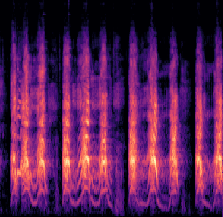
\includegraphics[width=3.2in,height=0.5in]{221.jpg}
\caption{Functions}
\end{figure}
\begin{figure} [h]
\centering
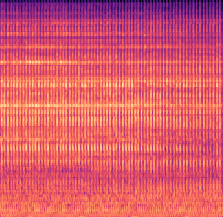
\includegraphics[width=4.3in,height=1.5in]{222.jpg}
\caption{Flows}
\end{figure}
\section{User Classes and Characteristics}
\begin{enumerate}
\item 一般使用者: 通過圖形化介面操作,可以輕鬆地完成辨識,分析有興趣的聲音
\item 城市管理者: 使用shell script批次實時監測並進行辨識
\item 家長: 架設錄音裝置,於嬰兒哭鬧時可獲得預警訊息
\end{enumerate}
\begin{figure} [h]
\centering
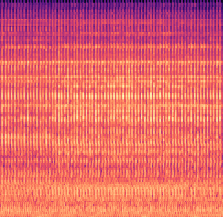
\includegraphics[width=4.6in,height=2.5in]{232.jpg}
\end{figure}
\begin{figure} [h]
\centering
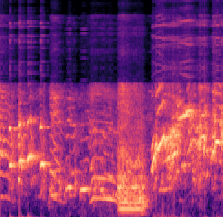
\includegraphics[width=5in,height=2.8in]{233.jpg}
\end{figure}
\section{Operating Environment}
\begin{enumerate}
\item OS: Windows 10
\item Python Runtime: version 3.6
\item Packages: run pip install -r requirements.txt
\item Tensorflow backend
\end{enumerate}

\section{Design and Implementation Constraints}
訓練模型時由於輸入圖片較大(512*512*1),建議可用GPU RAM在4GB或以上,否則會因頻繁重分配記憶體造成效率低下 由於model已經訓練好,使用者只要在Python環境下,安裝所需套件就可執行

\section{Assumptions and Dependencies}

\begin{center}
\begin{tabular}{|l|l|}
\hline \multicolumn{2}{|c|}{需自行安裝的套件:} \\\hline
pandas  & 讀取train.csv的label  \\ \hline
numpy  & 將原生list轉為更有效率的numpy.array用於訓練模型  \\ \hline
PIL  & 圖片讀取  \\\hline
scipy & 圖片處理 \\\hline
matplotlib  & 圖片與圖表視覺化呈現  \\\hline
librosa  & 音訊分析與處理  \\\hline
sklearn  & 調用one hot encoding, shuffle split  \\\hline
tensorflow  & keras底下引用的深度學習核心  \\\hline
keras  & 深度學習的高階API  \\
\hline \multicolumn{2}{|c|}{Python內建的:} \\\hline
tkinter       & GUI視窗介面  \\ \hline
pickle        & 保存資料  \\ \hline
os  & 讀取檔案  \\\hline

\end{tabular}
\end{center}

\chapter{External Interface Requirements}
\section{User Interfaces}
\begin{figure} 
\centering
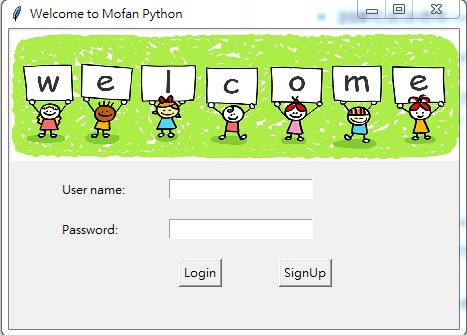
\includegraphics[width=3in,height=2.5in]{1.jpg}
\caption{使用者執行open_platform_final.py後,開啟tkinter視窗介面,有兩個按鈕: 
Login / SignUp}
\end{figure}
\begin{figure} [h]
\centering
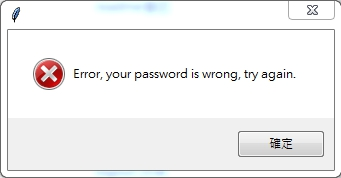
\includegraphics[width=3in,height=2in]{10.jpg}
\caption{當Password錯誤時會跳出密碼錯誤提示}
\end{figure}
\begin{figure} [h]
\centering
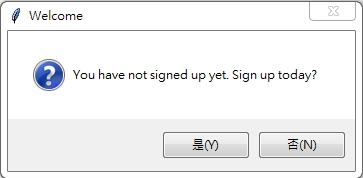
\includegraphics[width=2in,height=1.60in]{2.jpg}
\caption{當User name錯誤時會跳出註冊提示}
\end{figure}
\begin{figure} [h]
\centering
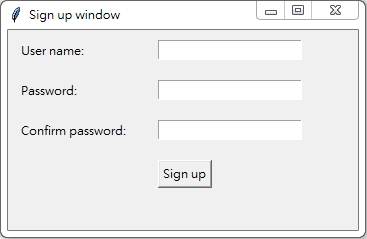
\includegraphics[width=3.2in,height=2.62in]{3.jpg}
\caption{接著進入註冊頁面}
\end{figure}
\begin{figure} [h]
\centering
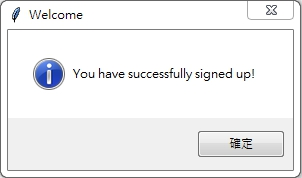
\includegraphics[width=2in,height=1.60in]{4.jpg}
\caption{當註冊成功就會跳出提示}
\end{figure}
\begin{figure} [h]
\centering
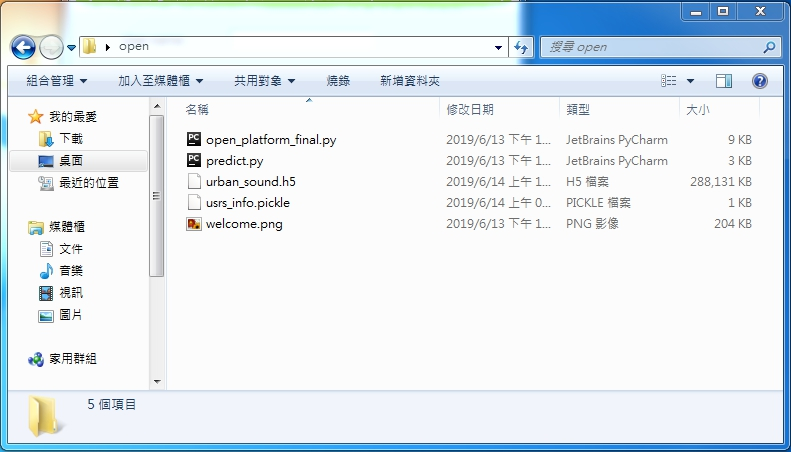
\includegraphics[width=4in,height=4in]{8.jpg}
\caption{同時會將帳號密碼存入usrs_info.pickle內}
\end{figure}
\begin{figure} [h]
\centering
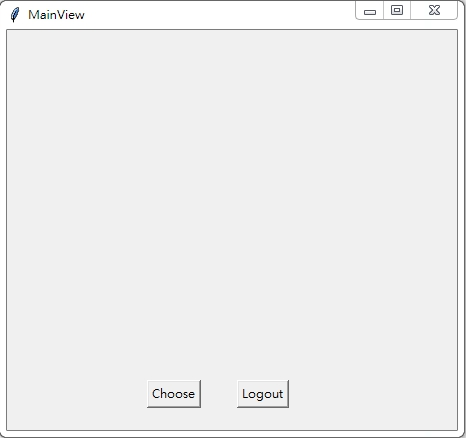
\includegraphics[width=3in,height=2in]{5.jpg}
\caption{接著登入成功進入主頁面,有兩個按鈕: Choose / LogOut}
\end{figure}

\begin{figure} [h]
\centering
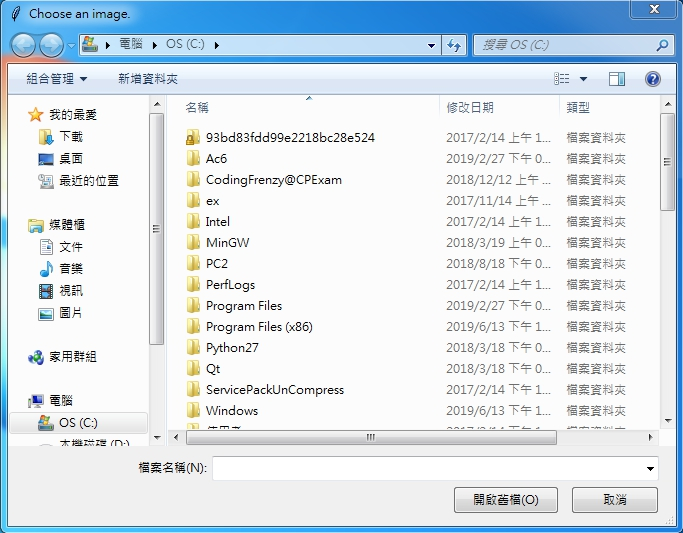
\includegraphics[width=3in,height=2in]{6.jpg}
\caption{點擊Choose選擇要辨識的音源檔}
\end{figure}
\begin{figure} [h]
\centering
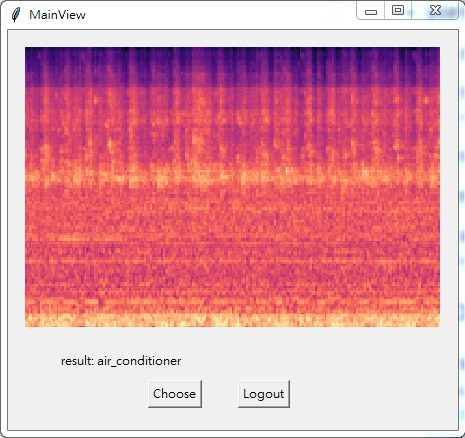
\includegraphics[width=3in,height=2in]{7.jpg}
\caption{接著就會出現頻譜以及判斷結果}
\end{figure}
\begin{figure} [h]
\centering
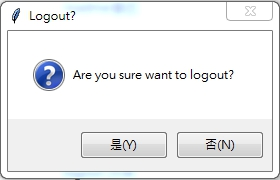
\includegraphics[width=1.77in,height=1.75in]{9.jpg}
\caption{點擊LogOut進行登出}
\end{figure}
\begin{figure} [h]
\centering
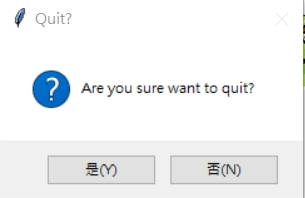
\includegraphics[width=2in,height=1.55in]{11.jpg}
\caption{關閉系統防呆}
\end{figure}
\clearpage
\section{Hardware Interfaces}
建議配備:
\begin{enumerate}
\item 作業系統: Windows 10 64 bit
\item 處理器: Intel Core i7-3770K
\item 記憶體: 8 GB 記憶體
\item 顯示卡: NVIDIA GTX 980Ti 2560x1440 or NVIDIA GTX 970 1920x1080
\item 最新的顯示卡驅動程式
\end{enumerate}

\section{Software Interfaces}
\begin{enumerate}
\item OS: Windows 10
\item Python Runtime: version 3.6
\item Packages: run pip install -r requirements.txt
\item Tensorflow backend
\end{enumerate}



\chapter{System Features}
\section{User Registration}
\subsection{Description and Priority}
概述為使用者如何去註冊,才可以使用這個系統\\
Priority – Medium

\subsection{Stimulus/Response Sequences}
\begin{center}
\begin{tabular}{|l|l|}\hline
系統反應動作使用 & 使用者操作動作  \\ \hline
 & a.使用者想要使用這系統  \\ \hline
b.系統回應需要先登入 &   \\\hline
 & c.使用者想登入按下登入按鈕  \\\hline
d.系統回應需要先註冊&   \\\hline
 & e.使用者想註冊按下註冊按鈕  \\\hline
f.系統彈出註冊視窗&   \\\hline
 & g.使用者輸入想要帳號密碼並按下確定  \\\hline
h.系統對比資料庫有無重複&   \\\hline
i.系統判定有重複並回傳重複訊息給使用者&   \\\hline
 & j.使用者重新輸入  \\\hline
k.系統對比資料庫有無重複&   \\\hline
l.系統判定無重複並進行註冊&   \\\hline
m.系統回傳註冊成功並跳回登入視窗	&   \\\hline
\end{tabular}
\end{center}

\subsection{Functional Requirements}
\begin{enumerate}
\item 使用者可以順利的註冊
\item 系統判定使用者輸入的帳密是否有重複
\item 如沒有重複,註冊成功並秀出訊息視窗
\item 當註冊成功,這個帳密可以登入
\end{enumerate}
\section{Administration}
\subsection{Description and Priority}
概述為在整個系統建立時,就有一個admin的帳號可以使admin不用註冊就可以登入使用系統\\
Priority – High
\subsection{Stimulus/Response Sequences}
\begin{center}
\begin{tabular}{|l|l|}\hline
系統反應動作使用 & 使用者操作動作  \\ \hline
 a.系統在創建時就已創建admin帳密資料&   \\ \hline
 & 	b.使用者想要使用這系統且有admin  \\\hline
 & c.使用者使用admin的帳密登入  \\\hline
d.系統判斷admin的帳密是否正確&   \\\hline
e.系統判定錯誤並回傳錯誤訊息給使用者	&   \\\hline
 & f.使用者重新輸入  \\\hline
g.系統判定正確,登入成功並進入主頁面視窗&   \\\hline
 & h.使用者開始使用	 \\\hline
\end{tabular}
\end{center}
\subsection{Functional Requirements}
\begin{enumerate}
\item 在創建系統時,就正確的創建admin的帳密,使監管者或是測試員可以直接登入
\item 可以判斷輸入的帳密是否與admin的帳密一致
\item 當admin的帳密輸入不一致,可以彈出帳密錯誤訊息的視窗
\item 當admin的帳密輸入正確即可以登入進入主頁面視窗
\end{enumerate}
\section{Login Logout system}
\subsection{Description and Priority}
概述為使用者如何登入和登出系統\\
Priority – Medium
\subsection{Stimulus/Response Sequences}
\begin{center}
\begin{tabular}{|l|l|}\hline
系統反應動作使用 & 使用者操作動作  \\ \hline
 & a.使用者想要使用這系統  \\ \hline
 & b.使用者使用自己的帳密登入  \\ \hline
d.系統對比資料庫有無這個帳號 &   \\\hline
e.系統判定無此帳號並回傳訊息給使用者 &   \\\hline
 & f.使用者重新輸入  \\\hline
g.系統對比資料庫有無這個帳號&   \\\hline
h.系統判定有此帳號並對比密碼是否一致&   \\\hline
i.系統判定密碼不一致並回傳訊息給使用者&   \\\hline
 & j.使用者重新輸入  \\\hline
g.系統對比資料庫有無這個帳號&   \\\hline
h.系統判定有此帳號並對比密碼是否一致&   \\\hline
i.系統判定密碼不一致並回傳訊息給使用者&   \\\hline
& j.使用者使用系統  \\\hline
 & k.使用者想登出並按下登出按紐		  \\\hline
l.系統接收登出訊息彈出是否登出訊息&   \\\hline
& m.使用者按下取消按紐	  \\\hline
 & n.使用者想登出並按下登出按紐  \\\hline
o.系統接收登出訊息彈出是否登出訊息&   \\\hline
 & p.使用者按下確定按紐   \\\hline
q.系統接收登出訊息,登出並回到登入視窗&   \\\hline
\end{tabular}
\end{center}
\subsection{Functional Requirements}
\begin{enumerate}
\item 可以判定是否有除了admin外的使用者帳密
\item 如沒有除了admin外的使用者帳密,可以切換到註冊系統
\item 可以判斷輸入的帳密是否與資料庫內的帳密一致
\item 當使用者輸入的帳密與資料庫內的帳密不一致,可以彈出帳密錯誤訊
\item 當使用者的帳密輸入正確即可以登入進入主頁面視窗
\item 登出按鈕,可以正確的彈出確認訊息視窗
\item 當確認訊息視窗按下取消,可以正確的回到原本畫面
\item 當確認訊息視窗按下確定,可以正確的登出並回到登入系統
\end{enumerate}
\section{Main Request System}
\subsection{Description and Priority}
概述為主要系統運作,如何去選定要判別的png和wav檔,並輸出結果\\
Priority – Very High
\subsection{Stimulus/Response Sequences}
\begin{center}
\begin{tabular}{|l|l|}\hline
系統反應動作使用 & 使用者操作動作  \\ \hline
 a.登入成功跳轉到主頁面視窗&   \\ \hline
 & b.使用者按下choose按鈕  \\ \hline
d.系統對比資料庫有無這個帳號 &   \\\hline
e.系統判定無此帳號並回傳訊息給使用者 &   \\\hline
 & f.使用者重新輸入  \\\hline
g.系統對比資料庫有無這個帳號&   \\\hline
h.系統判定有此帳號並對比密碼是否一致&   \\\hline
i.系統判定密碼不一致並回傳訊息給使用者&   \\\hline
 & j.使用者重新輸入  \\\hline
g.系統對比資料庫有無這個帳號&   \\\hline
h.系統判定有此帳號並對比密碼是否一致&   \\\hline
i.系統判定密碼不一致並回傳訊息給使用者&   \\\hline
& j.使用者使用系統  \\\hline
 & k.使用者想登出並按下登出按紐		  \\\hline
l.系統接收登出訊息彈出是否登出訊息&   \\\hline
& m.使用者按下取消按紐	  \\\hline
 & n.使用者想登出並按下登出按紐  \\\hline
o.系統接收登出訊息彈出是否登出訊息&   \\\hline
 & p.使用者按下確定按紐   \\\hline
q.系統接收登出訊息,登出並回到登入視窗&   \\\hline
\end{tabular}
\end{center}
\subsection{Functional Requirements}
\begin{enumerate}
\item 按下choose按鈕可以正確地彈出選擇檔案視窗
\item 可以正確的選擇想要的檔案至程式
\item 可以正確的判斷選擇的檔案是音訊或是圖片檔
\item 如不是音訊或是圖片檔,可以輸出找不到檔案到視窗上
\item 可以讀取音訊檔並轉成頻譜圖
\item 可以讀取轉好或預先選定的頻譜圖
\item 可以使用預先訓練好的model分析預測頻譜圖的屬性
\item 可以輸出頻譜圖到視窗上
\item 可以輸出預測結果到視窗上
\end{enumerate}
\chapter{Other Nonfunctional Requirements}
\section{Performance Requirements}
\begin{enumerate}
\item 每次辨識必須在0.1秒完成(讓real-time辨識得以實現)\\
如下圖,辨識頻譜圖時每次花費時間皆在0.07秒左右,符合需求
\begin{figure}[H]
\centering
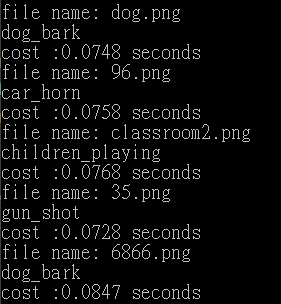
\includegraphics[width=2in,height=2.2in]{time1.PNG}
\end{figure}
如下圖,辨識音檔時因需轉檔,費時在0.5至2秒間,超出需求
\begin{figure}[H]
\centering
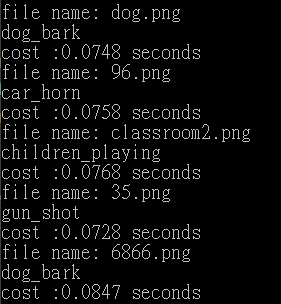
\includegraphics[width=2in,height=2.2in]{time1.PNG}
\end{figure}
\item 準確率(預測結果等於實際值)必須在70\%以上
\begin{center}
\begin{tabular}{|l|l|}
\hline \multicolumn{2}{|c|}{使用網路資源與自行錄製音訊測試} \\\hline
實際值  & 辨識值  \\ \hline
dog_bark  & dog_bark  \\ \hline
drilling  & unknow  \\ \hline
engine_idling  & engine_idling  \\ \hline
siren  & siren  \\ \hline
children_playing  &children_playing   \\ \hline
\end{tabular}
\end{center}
實測5個來源、長度各異的音檔,準確率80\%
\end{enumerate}

\section{Safety Requirements}
\begin{enumerate}
\item file防呆(只能選定.png或是.wav)
\begin{figure}[H]

\includegraphics[width=3.2in,height=1in]{520.PNG}
\end{figure}
\item 檢查帳號避免重複註冊
\begin{figure}[H]
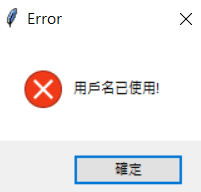
\includegraphics[width=2in,height=2.1in]{521.PNG}
\end{figure}
\item 檢查帳密是否正確
\begin{figure}[H]
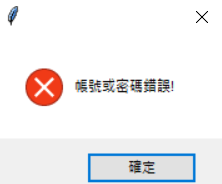
\includegraphics[width=2in,height=2.1in]{522.PNG}
\end{figure}
\end{enumerate}

\section{Security Requirements}
使用pickle檔存使用者帳密,pickle檔提供了一個簡單的持久化功能。可以將對象以文件的形式存放在磁盤上,用pickle來序列化使得存使用者帳密不會直接洩漏


\end{CJK*}
\end{document}
